\chapter{Progettazione concettuale}
\section{Introduzione}
In questa sezione verrà introdotta la progettazione concettuale dell'applicativo. Partendo da un primo diagramma di classe in UML. Dal risultato dell'analisi dei requisiti che devono essere soddisfatti si arriverà a uno schema concettuale ristrutturato. Saranno evidenziati i concetti rilevanti ai fini della rappresentazione dei dati e le relazioni che intercorrono tra di esse.

\section{Class Diagram}
\begin{figure}[!h]
    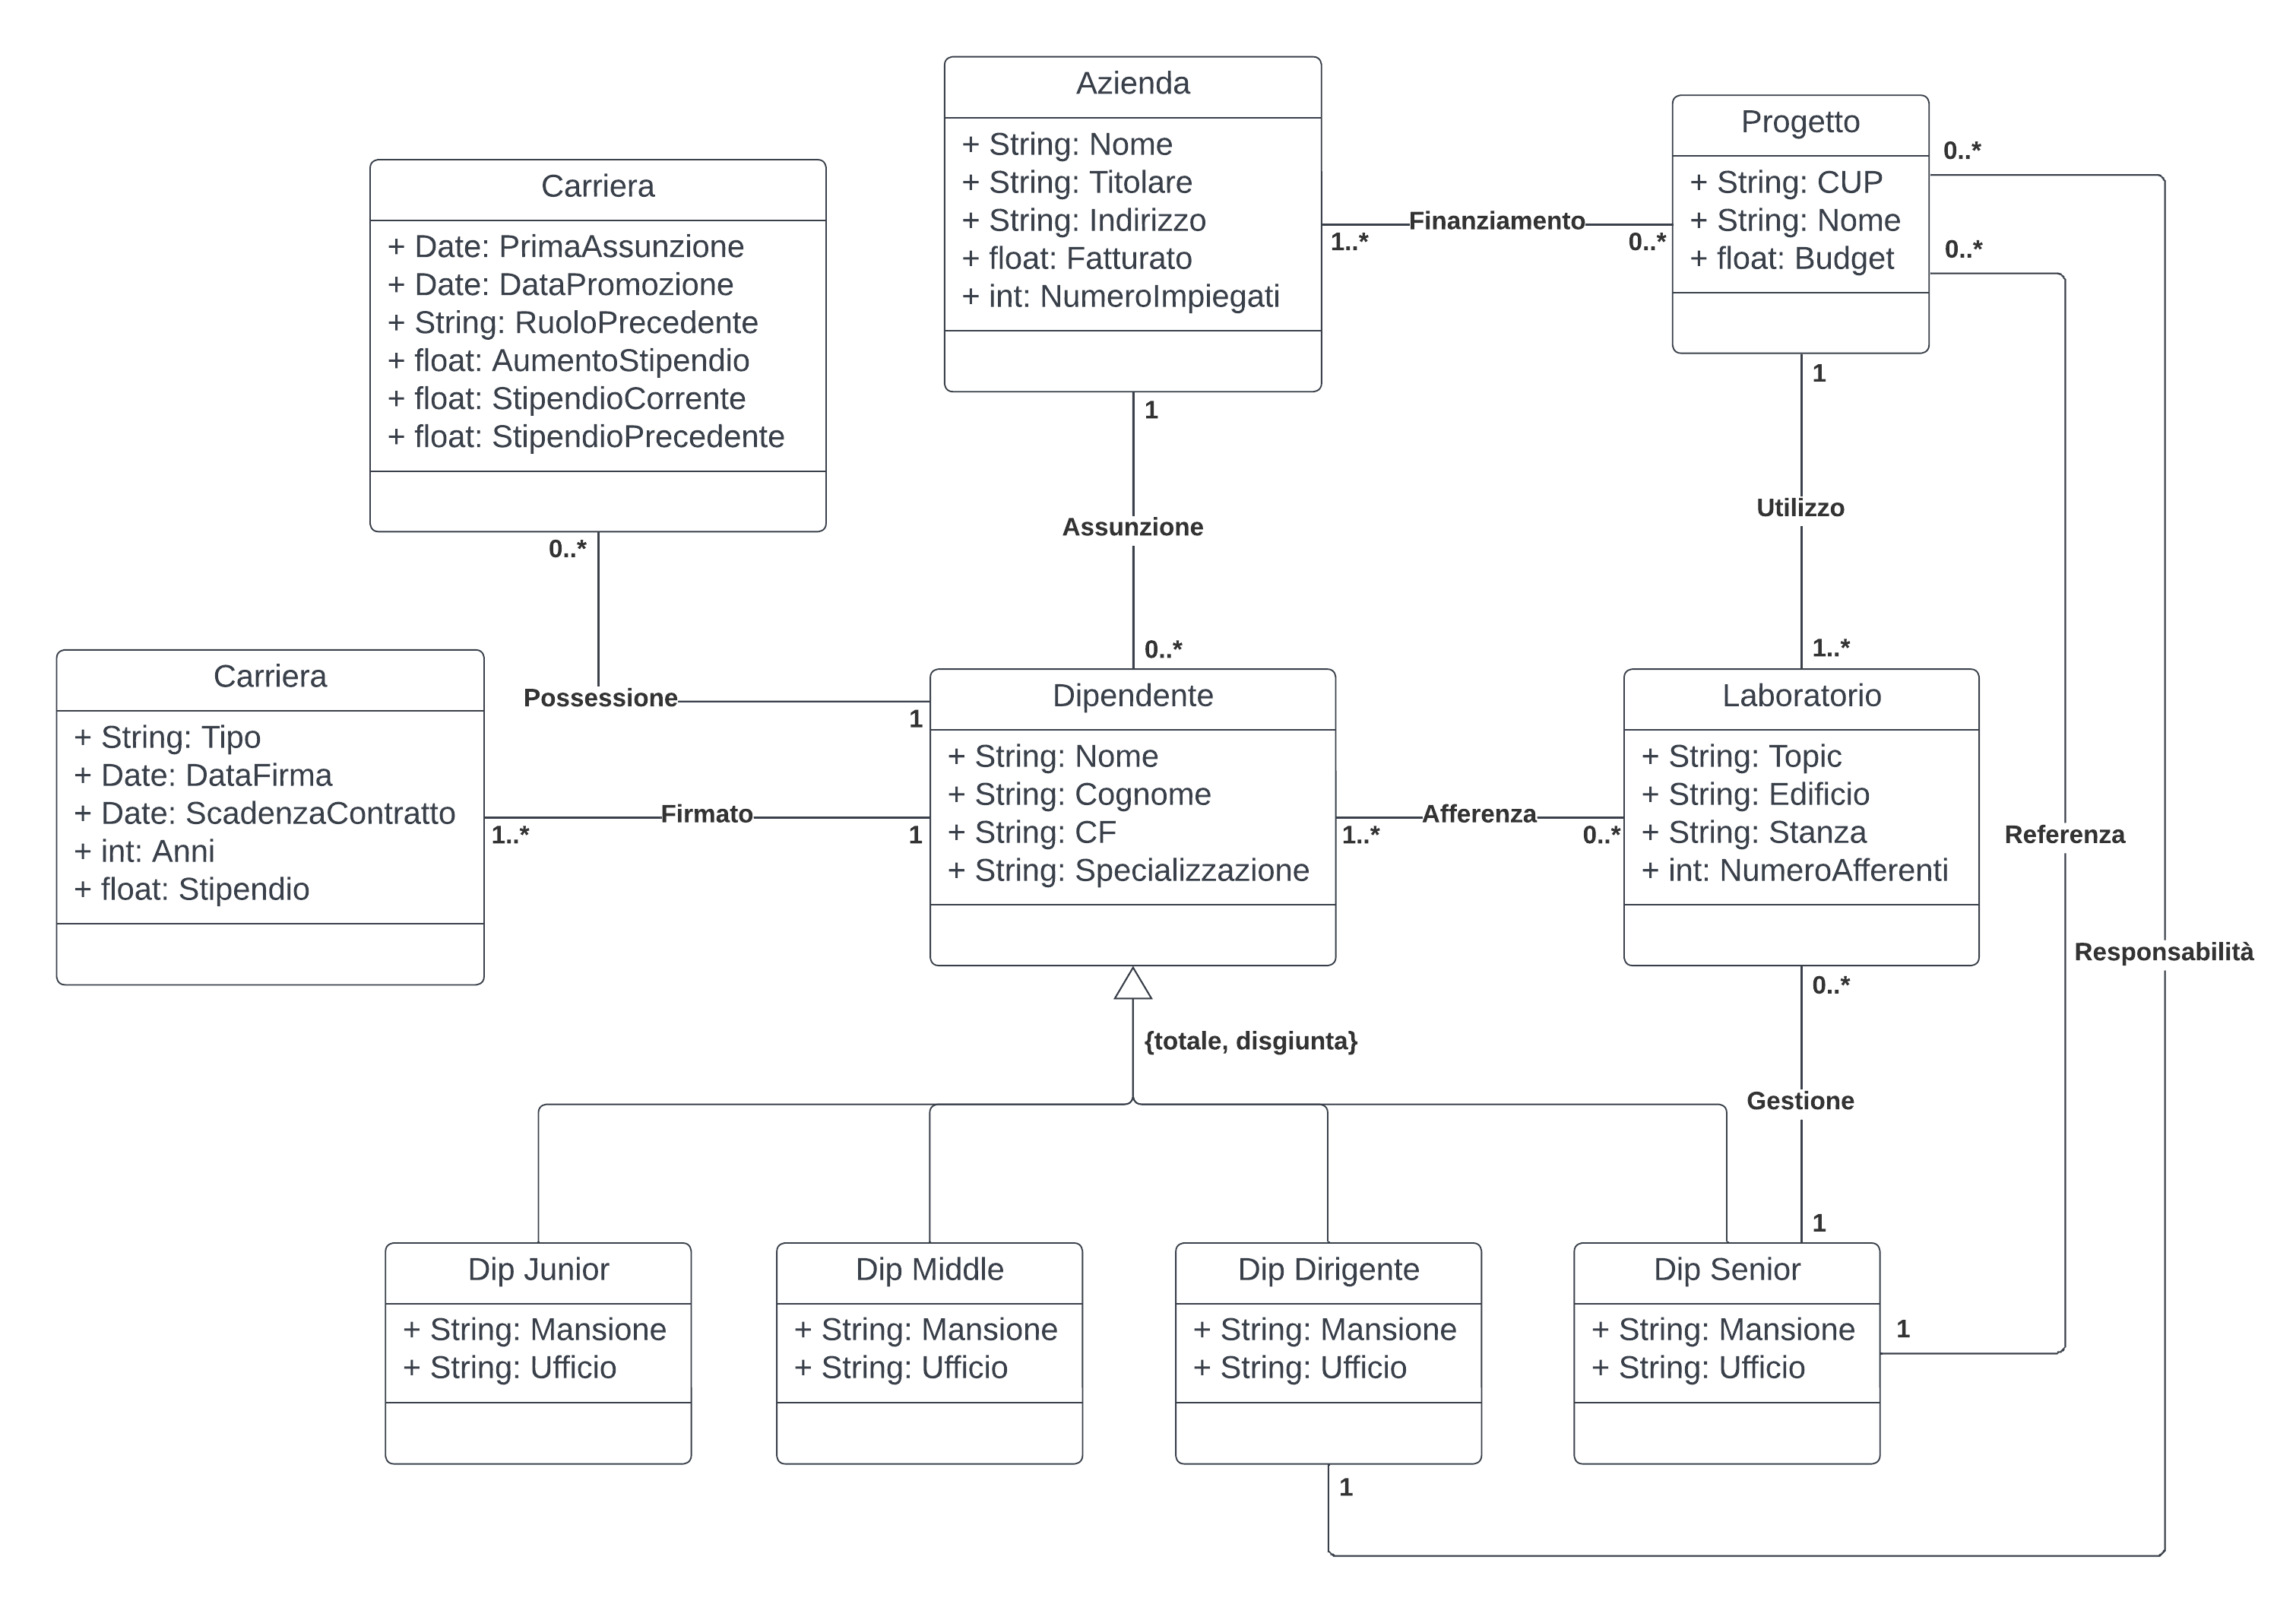
\includegraphics[width=.8\linewidth]{./Immagini/BozzaProgetto.png}
\end{figure}

\section{Ristrutturazione del Class Diagram}
Al fine di rendere il class diagram idoneo alla traduzione logica e di migliorare l’efficienza dell’implementazione si procede alla ristrutturazione dello stesso.

\subsection{Analisi delle ridondanze}
Sono ora anlizzate le ridondanze trovate all'interno del Class Diagram precedente:
\begin{itemize}
    \item Il numero degli impiegati può essere ricavato attraverso la relazione assunzione,
    \item Il numero di anni di contratto può essere ricavato sottraendo alla data di scadenza la data di assunzione,
    \item Il numero di afferenti di un laboratorio può essere ricavato contando i dipendenti dalla relazione Afferenza.
\end{itemize}
Da ricordare che la rimozione delle ridondanze è specifica alla progettazione concettuale: in fase di implementazione potrebbe rivelarsi conveniente introdurre alcuni attributi ridondanti al fine di facilitare le query (un esempio sono StipendioPrecedente e StipendioCorrente).

\subsection{Analisi degli identificativi}
Per facilitare la traduzione verso lo schema logico e per il recupero efficiente dei dati si inseriscono gli identificativi IDContratto e IDCarriera, rispettivamente alle entità Contratto e Carriera.
Per identificare univocamente i dipendenti sarà considerato unico il codice fiscale. Per l'azienda sono presi come identificativi il nome e la via, mentre per il progetto sarà utilizzato il CUP. Infine per il laboratorio si possono considerare univoci nel sistema tutti i suoi attributi, ovvero "Topic, Edificio, Stanza".


\subsection{Rimozione degli attributi multivalore}
Il nome e il cognome del titolare dell'azienda saranno considerati come una stringa unica.

\subsection{Rimozione degli attributi composti}
Nell'entità Azienda l'attributo Indirizzo sarà estratto in modo da delineare gli attributi: "Via, Civico, CAP".

\subsection{Partizione/Accorpamento delle associazioni}
Non vengono eseguiti accorpamenti o partizioni delle associazioni.

\subsection{Rimozione delle gerarchie}
La disgiunzione totale tra la superclasse Dipendente e le sottoclassi Dipendente Junior, Dipendente Middle, Dipendente Senior e Dipendente Dirigente viene eliminata accorpando le sottoclassi nella superclasse: sarà necessario inserire un attributo "Ruolo" per controllare la categoria del dipendente.\\
Sarà anche necessario modificare le molteplicità delle associazioni tra la classe Dipendente e le classi Progetto e Laboratorio.
\newpage
\section{Diagrammi ristrutturati}
\subsection{Class Diagram}
\begin{figure}[!h]
    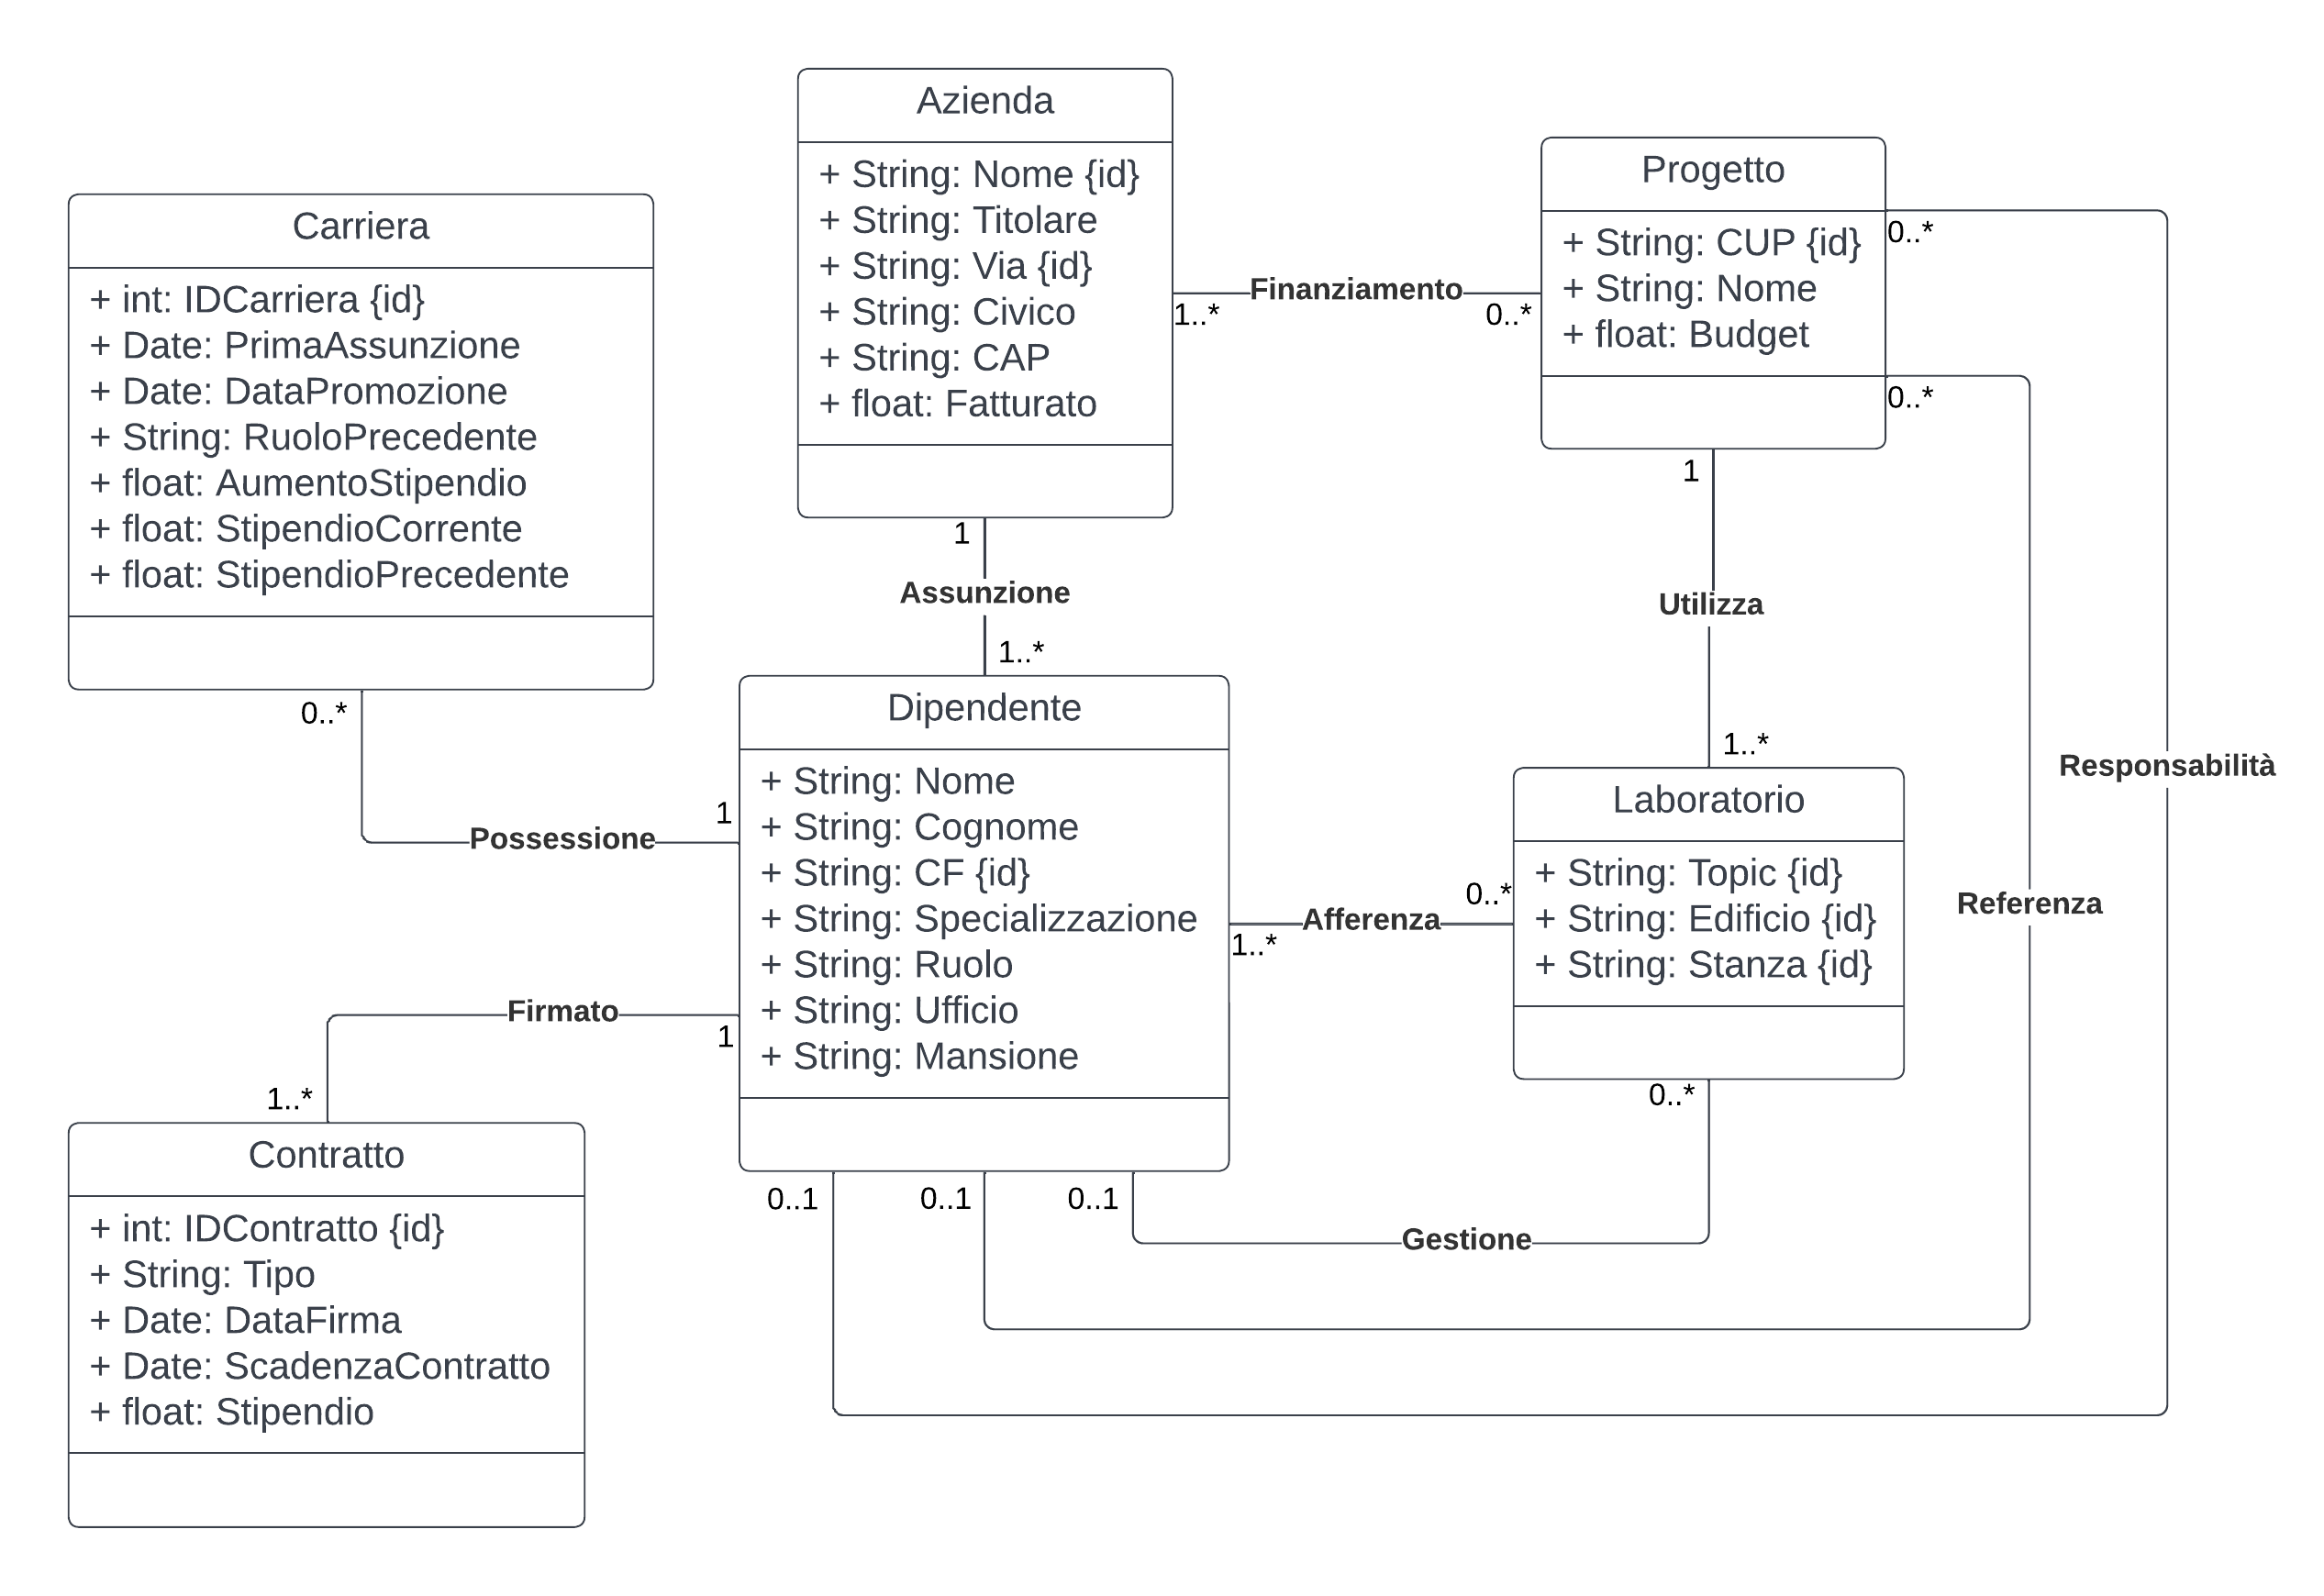
\includegraphics[width=.8\linewidth]{./Immagini/Ristrutturato.png}
\end{figure}
\subsection{Diagramma ER}
\begin{figure}[!h]
    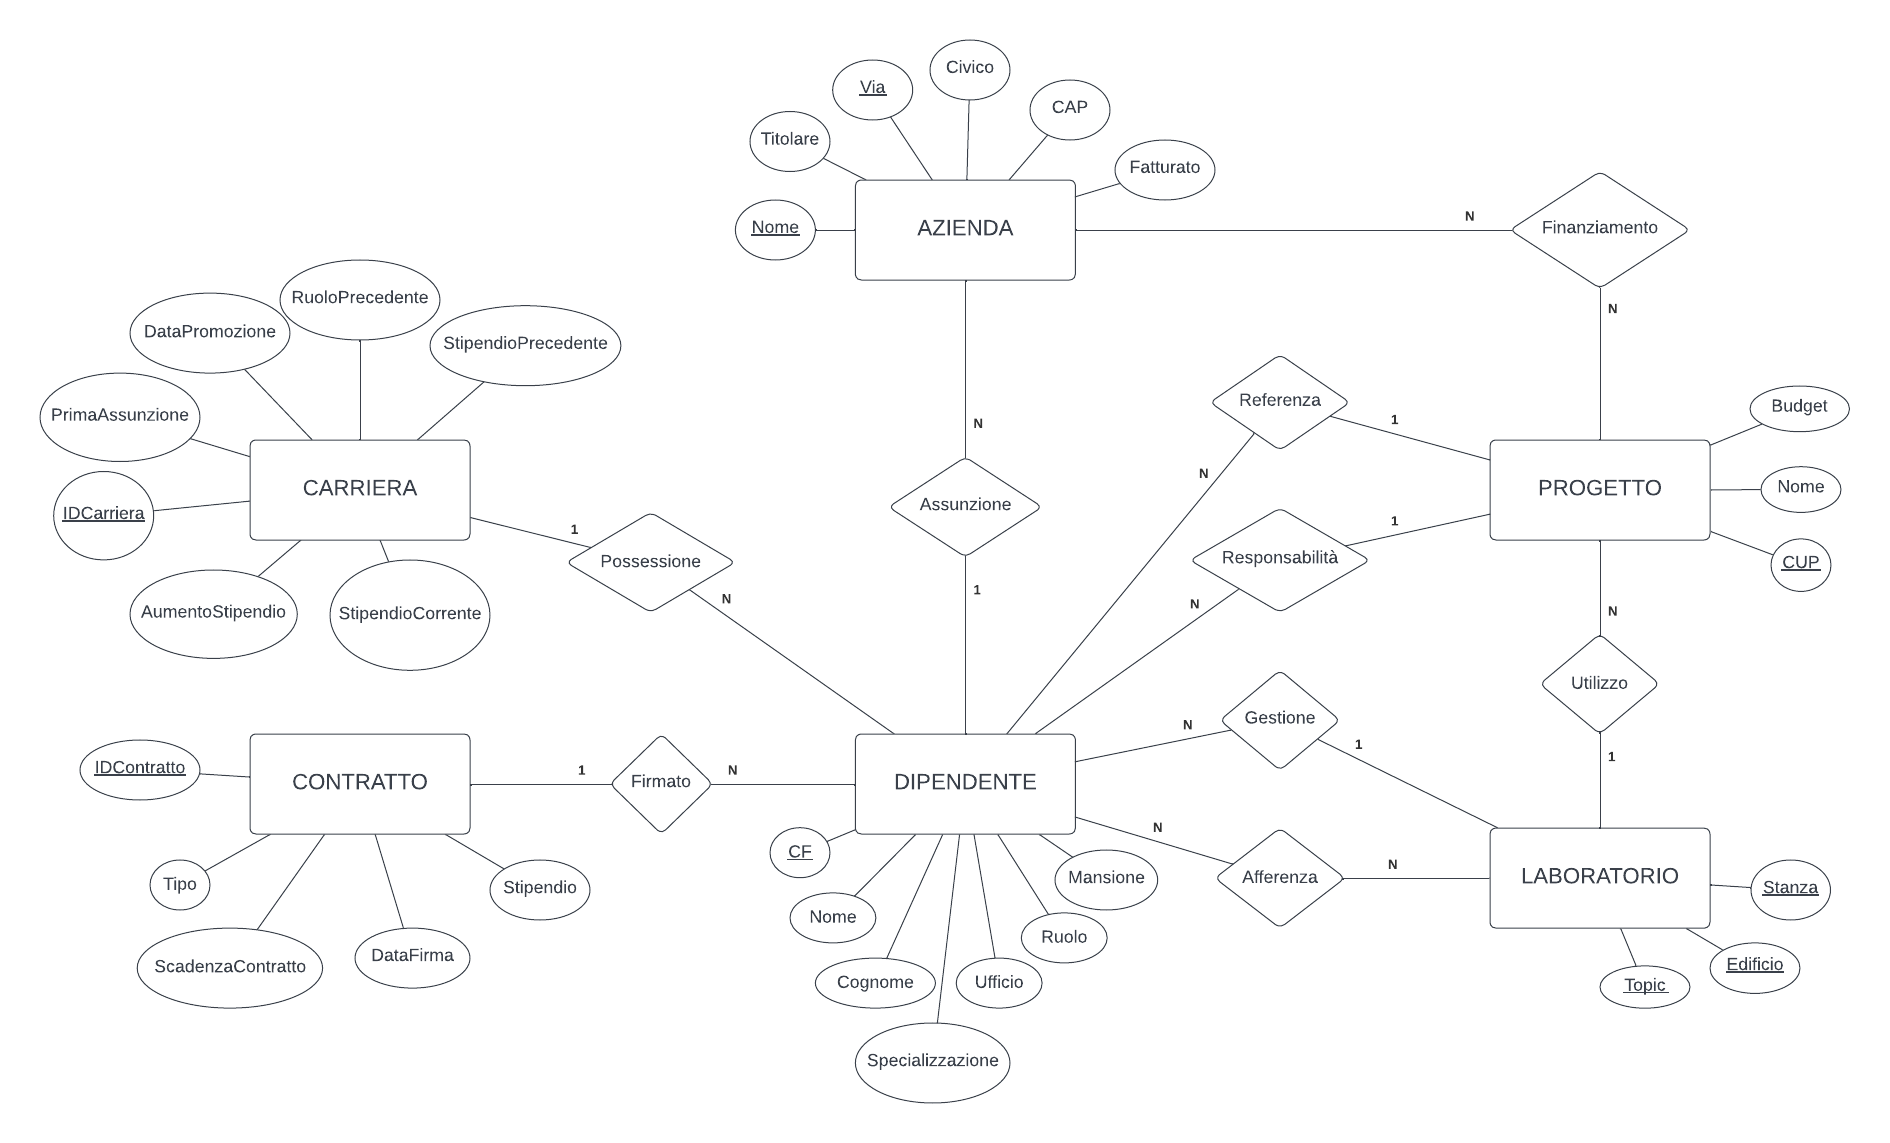
\includegraphics[width=.8\linewidth]{./Immagini/ER.png}
\end{figure}